\documentclass[svgnames,
               hyperref={colorlinks,citecolor=DeepPink4,linkcolor=FireBrick,urlcolor=Maroon},
               usepdftitle=false]  % see \hypersetup{} below
               {beamer}

\mode<presentation>{
  \usetheme{Madrid}
  %\usecolortheme{seagull}
  \usecolortheme{seagull}
  \setbeamercovered{transparent}
  \setbeamerfont{frametitle}{size=\large}
}

\setbeamercolor*{block title}{bg=red!10}
\setbeamercolor*{block body}{bg=red!5}

%\usepackage[svgnames]{xcolor}
\usepackage{hyperref}
\hypersetup{
    pdftitle = {3 research overview slides},
    pdfauthor = {Ed Bueler},
    pdfsubject = {},
    pdfkeywords = {}
}

\usepackage[english]{babel}
\usepackage[latin1]{inputenc}
\usepackage{times}
\usepackage[T1]{fontenc}
\usepackage{empheq,bm,xspace,fancyvrb,soul}
\usepackage{tikz}
\usetikzlibrary{shapes,arrows.meta,decorations.markings,decorations.pathreplacing,fadings,positioning}
\usepackage[kw]{pseudo}
\pseudoset{left-margin=15mm,topsep=5mm,label=,idfont=\texttt,st-left=,st-right=}

\makeatletter
%\newcommand\notsotiny{\@setfontsize\notsotiny\@vipt\@viipt}
\newcommand\notsotiny{\@setfontsize\notsotiny\@viipt\@viiipt}
\makeatother

\newcommand{\eps}{\epsilon}
\newcommand{\RR}{\mathbb{R}}

\newcommand{\grad}{\nabla}
\newcommand{\Div}{\nabla\cdot}
\newcommand{\trace}{\operatorname{tr}}

\newcommand{\hbn}{\hat{\mathbf{n}}}

\newcommand{\bb}{\mathbf{b}}
\newcommand{\be}{\mathbf{e}}
\newcommand{\bbf}{\mathbf{f}}
\newcommand{\bg}{\mathbf{g}}
\newcommand{\bn}{\mathbf{n}}
\newcommand{\bq}{\mathbf{q}}
\newcommand{\br}{\mathbf{r}}
\newcommand{\bu}{\mathbf{u}}
\newcommand{\bv}{\mathbf{v}}
\newcommand{\bw}{\mathbf{w}}
\newcommand{\bx}{\mathbf{x}}

\newcommand{\bF}{\mathbf{F}}
\newcommand{\bQ}{\mathbf{Q}}
\newcommand{\bU}{\mathbf{U}}
\newcommand{\bV}{\mathbf{V}}
\newcommand{\bX}{\mathbf{X}}

\newcommand{\btau}{\bm{\tau}}
\newcommand{\bxi}{\bm{\xi}}

\newcommand{\bzero}{\bm{0}}

\newcommand{\cK}{\mathcal{K}}
\newcommand{\cV}{\mathcal{V}}

\newcommand{\rhoi}{\rho_{\text{i}}}

\newcommand{\ip}[2]{\left<#1,#2\right>}

\newcommand{\nn}{{\text{n}}}
\newcommand{\pp}{{\text{p}}}
\newcommand{\qq}{{\text{q}}}
\newcommand{\rr}{{\text{r}}}

\newcommand{\ds}{\displaystyle}

\newcommand{\bus}{\bu|_s}
\newcommand{\oo}[1]{\displaystyle O\left(#1\right)}
\newcommand{\sold}{s_{\text{o}}}

\newcommand{\maxR}{R^{\bm{\oplus}}}
\newcommand{\minR}{R^{\bm{\ominus}}}
\newcommand{\iR}{R^{\bullet}}

\newcommand{\sdoi}[1]{\,{\tiny \href{https://doi.org/#1}{doi:#1}}}



\title{Ed Bueler's research in 3 slides}

%\subtitle{\emph{}}

%\author{Ed Bueler}

\institute[]{Department of Mathematics \& Statistics \\ University of Alaska Fairbanks}

\date[]{\footnotesize August 2024}

%\titlegraphic{\begin{picture}(0,0)
%    \put(0,180){\makebox(0,0)[rt]{
\includegraphics[width=4cm]{figs/software.png}}}
%  \end{picture}
%}

\titlegraphic{
\includegraphics[width=0.25\textwidth]{figs/uafbw.png} \hfill}

%% to start section counter at 0 see
%% https://tex.stackexchange.com/questions/170222/change-the-numbering-in-beamers-table-of-content

\setbeamertemplate{page number in head/foot}[appendixframenumber]

\begin{document}
\addtocounter{framenumber}{-1}

\beamertemplatenavigationsymbolsempty

{
  %\usebackgroundtemplate{\includegraphics[width=\paperwidth]{../talk-oxford/images/gray-british-clark2022.png}}
  \begin{frame}

\vspace{10mm}

    \titlepage
  \end{frame}
}


\begin{frame}{thread 1: numerical models of glaciers and ice sheets}

\begin{columns}
\begin{column}{0.45\textwidth}
\begin{itemize}
\item I work on {\color{FireBrick} numerical models of glaciers and ice sheets}
\item mathematical and computational aspects
\item \textbf{results:}
    \begin{enumerate}
    \item 2023 paper on ice sheet model performance scaling    
    \item I was a lead author of the \,\,\raisebox{-9pt}[9mm]{\href{https://www.pism.io/}{
\includegraphics[width=0.45\textwidth]{figs/pism.png}}}
    \end{enumerate}

\end{itemize}
\end{column}
\begin{column}{0.55\textwidth}
\hfill 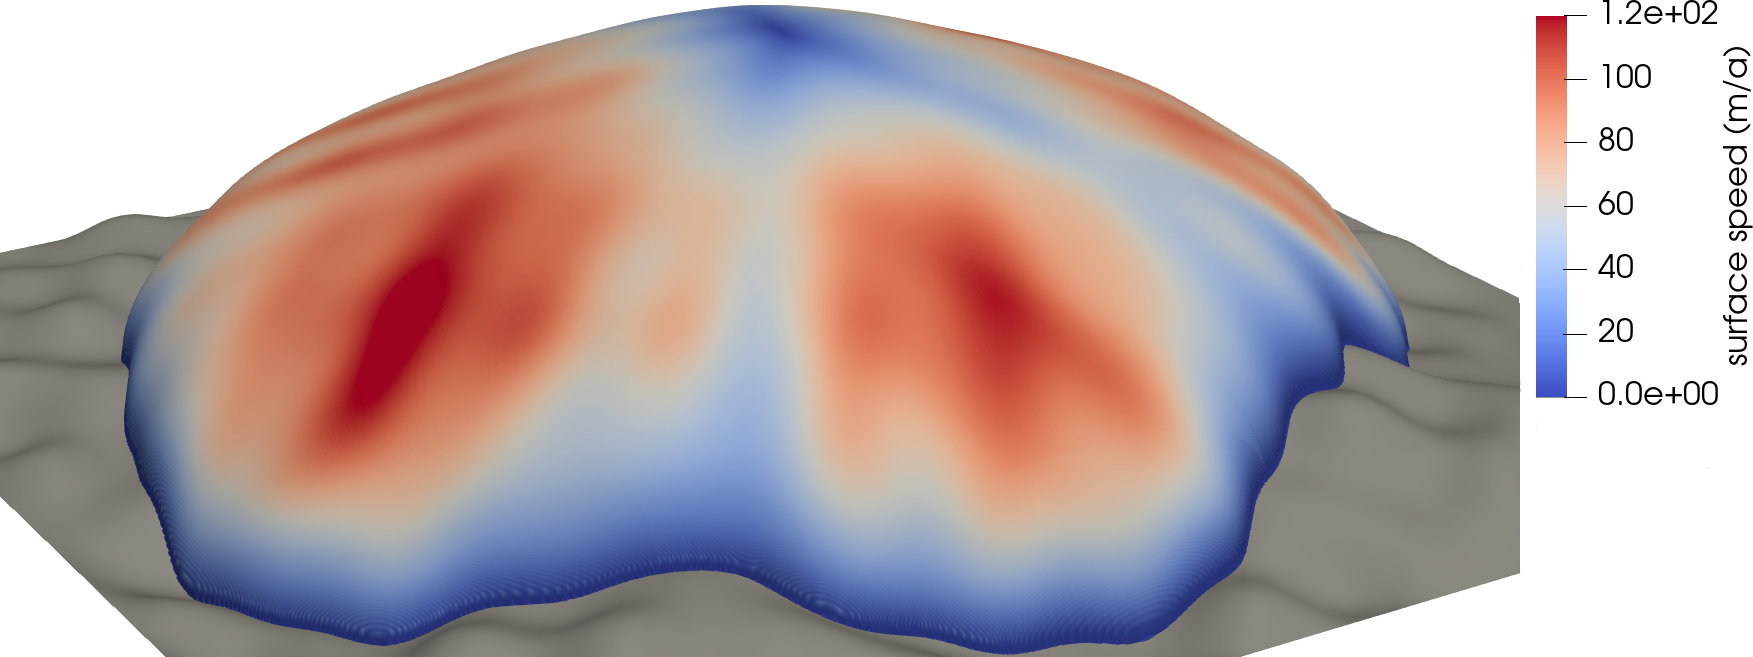
\includegraphics[width=\textwidth]{figs/sialev8scene.png}

\vspace{5mm}
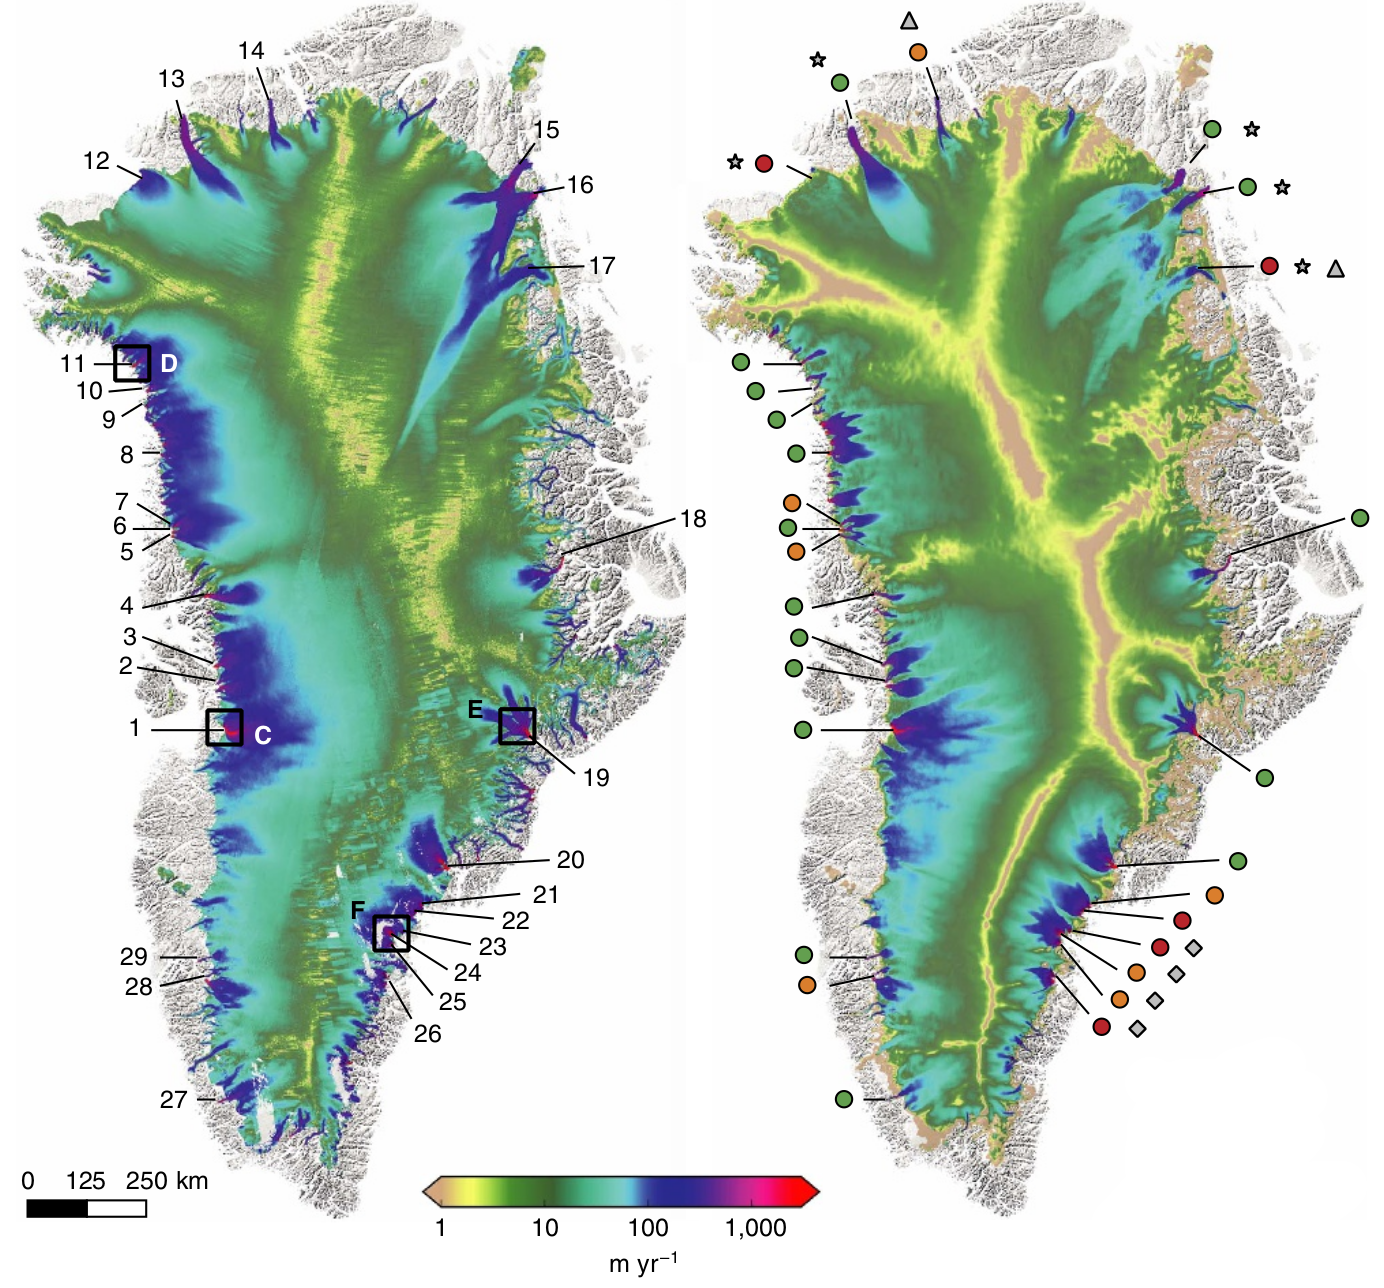
\includegraphics[width=0.75\textwidth]{figs/gis-aschwanden2016.png}

\vspace{-11mm}
\hfill {\tiny 2023 paper $\to$} \quad \href{https://doi.org/10.1017/jog.2022.113}{
\includegraphics[width=0.22\textwidth]{figs/QRperformance.png}}
\end{column}
\end{columns}
\end{frame}


\begin{frame}{thread 2: multigrid solvers for free-boundary problems}

\begin{columns}
\begin{column}{0.6\textwidth}
\begin{itemize}
\item I work on {\color{FireBrick} free-boundary problems}, which are partial differential equations (PDEs) wherein boundary conditions apply at locations only known after you solve the problem
    \begin{itemize}
    \item[$\circ$] rephrase as variational inequalities or complementarity problems
    \end{itemize}
\item \textbf{result:} a new {\color{FireBrick} multigrid solver} for variational inequalities
    \begin{itemize}
    \item[$\circ$] joint work with P.~Farrell (Oxford)
    \item[$\circ$] implemented in the \,\raisebox{-4pt}[3mm][3mm]{\href{https://www.firedrakeproject.org/index.html}{
\includegraphics[width=0.35\textwidth]{figs/firedrakebanner.png}}}\, finite element library (Python)
    \end{itemize}
\end{itemize}
\end{column}
\begin{column}{0.4\textwidth}
{\centering

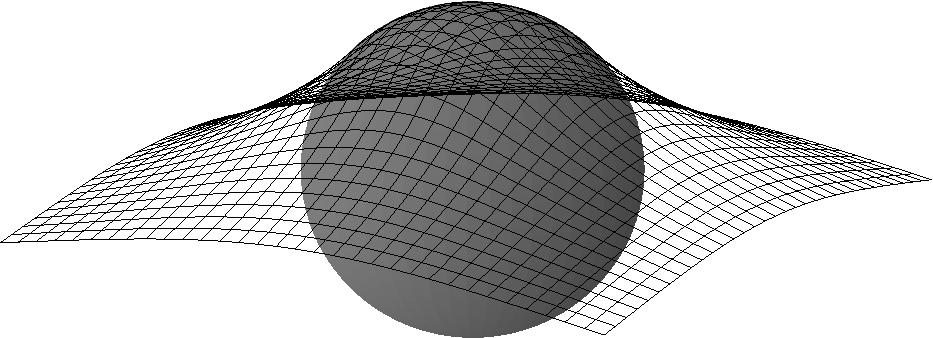
\includegraphics[width=\textwidth]{figs/obstacle65.pdf}

\vspace{5mm}

\includegraphics[width=\textwidth]{figs/mg-grids.png}

{\tiny
\hspace{3mm} $\Omega^3$ \hspace{9mm} $\Omega^2$ \hspace{9mm} $\Omega^1$ \hspace{9mm} $\Omega^0$ \hspace{1mm}
}

\vspace{5mm}
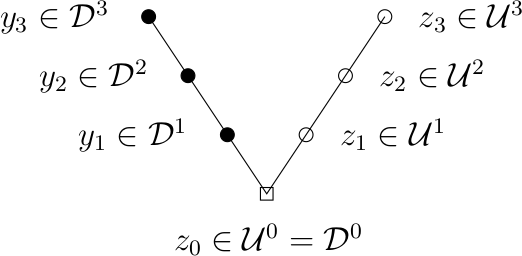
\includegraphics[width=0.7\textwidth]{figs/fascd-vcycle.png}\par}

\vspace{5mm}
\hfill {\tiny 2024 paper $\to$} \quad \href{https://epubs.siam.org/doi/10.1137/23M1594200}{
\includegraphics[width=0.3\textwidth]{figs/QRbuelerfarrell.png}}
\end{column}
\end{columns}
\end{frame}


\begin{frame}{thread 3: new book on mathematics of HPC}

\begin{columns}
\begin{column}{0.6\textwidth}
\begin{itemize}
\item I teach numerical analysis, numerical linear algebra, differential equations, and optimization at the MS level
\item students (and researchers) in these areas have few resources for tackling the 21st century:
    \begin{itemize}
    \item[$\circ$] {\color{FireBrick} mathematical solver concepts} based on matrices and function spaces
    \item[$\circ$] {\color{FireBrick} high performance computing libraries} in performant languages like C
    \end{itemize}
\item \textbf{result:} published {\color{FireBrick} new book} on solving PDE problems using the \,\raisebox{-3pt}[4.5mm]{\href{https://petsc.org/release/}{
\includegraphics[width=0.3\textwidth]{figs/petsc.png}}}\, solver library
\end{itemize}
\end{column}
\begin{column}{0.4\textwidth}
\vspace{2mm}

\hfill \href{https://epubs.siam.org/doi/book/10.1137/1.9781611976311}{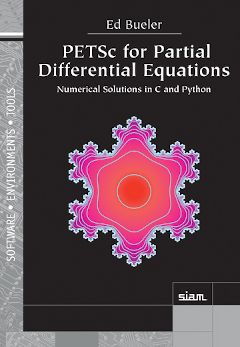
\includegraphics[width=0.75\textwidth]{figs/frontcover.jpg}}

\vspace{10mm}
\hfill {\tiny 2021 book $\to$} \quad \href{https://epubs.siam.org/doi/book/10.1137/1.9781611976311}{
\includegraphics[width=0.3\textwidth]{figs/QRbook.png}}
\end{column}
\end{columns}
\end{frame}

\end{document}
